\section{src/mlpack/core.hpp File Reference}
\label{core_8hpp}\index{src/mlpack/core.\+hpp@{src/mlpack/core.\+hpp}}


Include all of the base components required to write M\+L\+P\+A\+CK methods, and the main M\+L\+P\+A\+CK Doxygen documentation.  


Include dependency graph for core.\+hpp\+:
\nopagebreak
\begin{figure}[H]
\begin{center}
\leavevmode
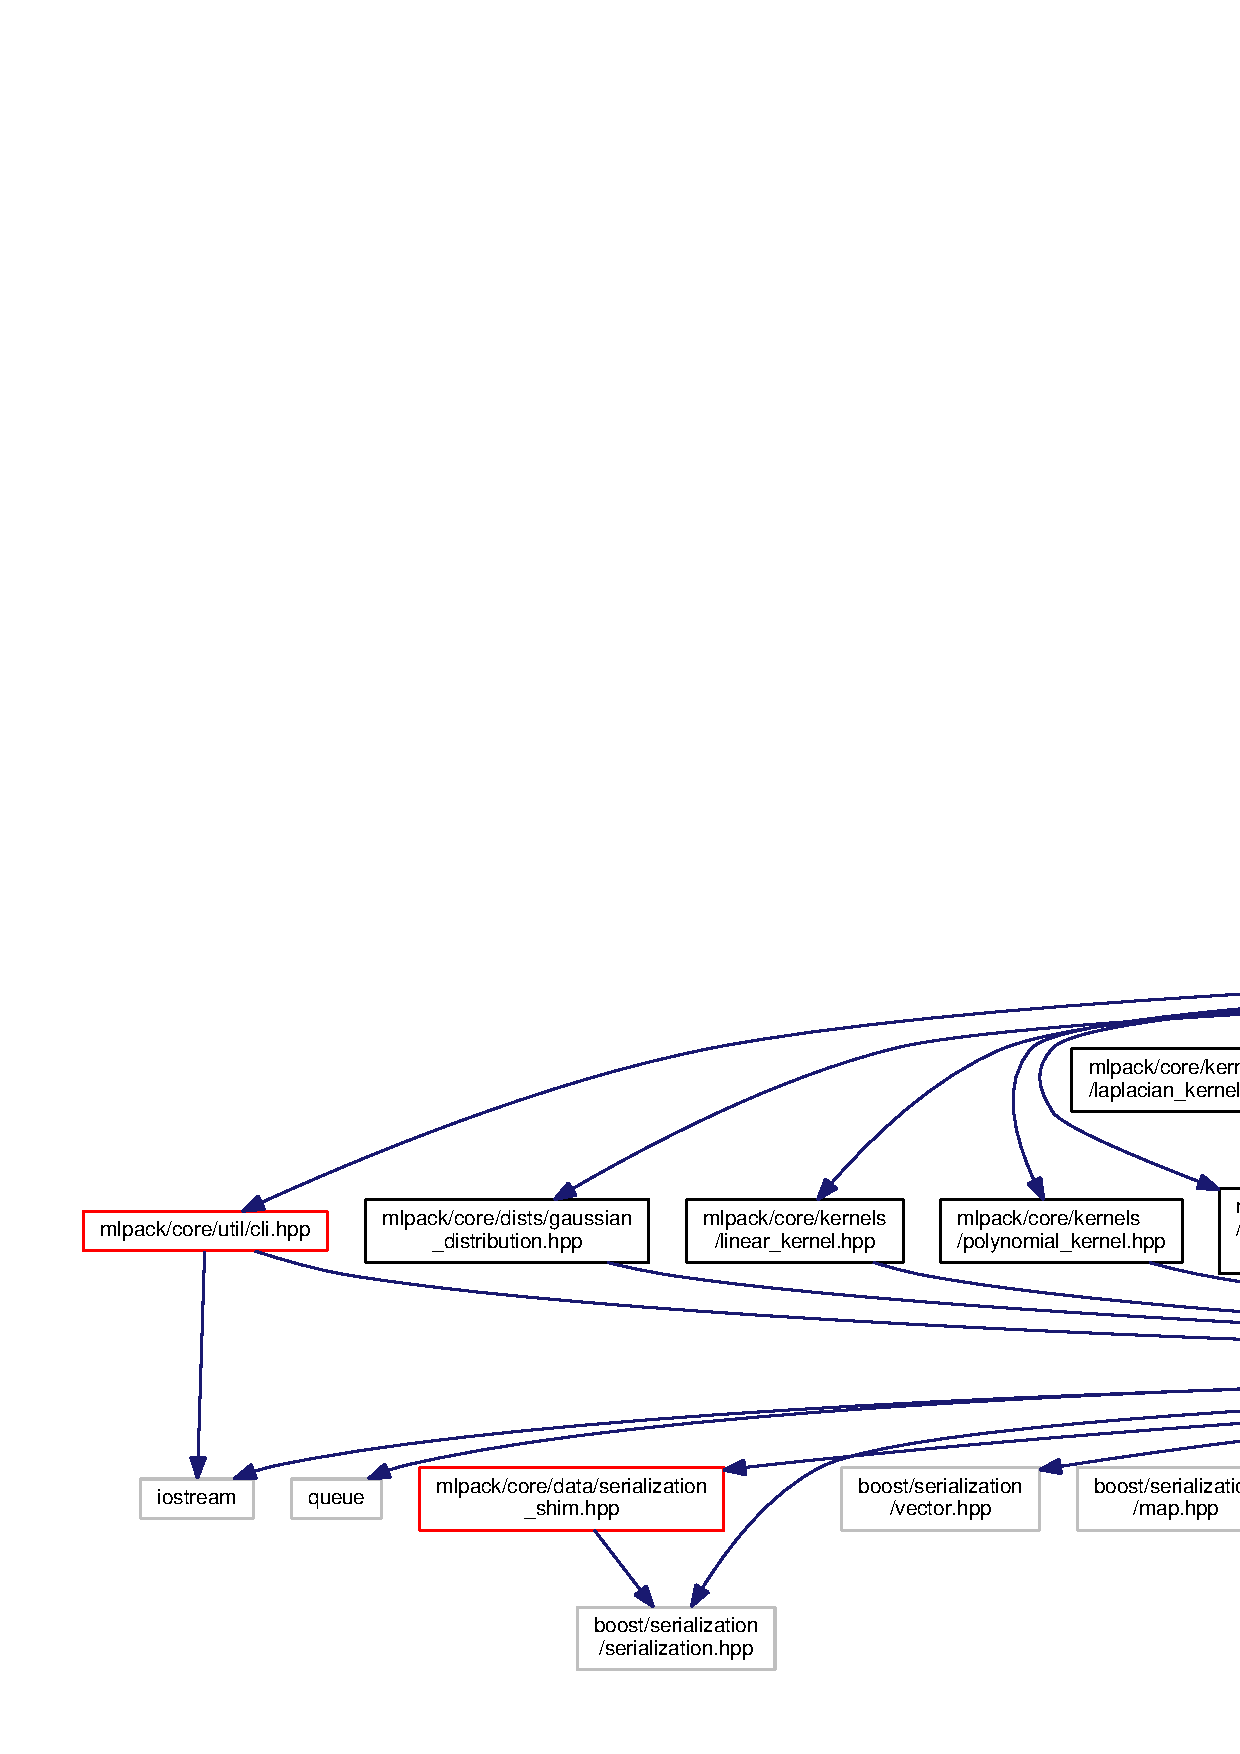
\includegraphics[width=350pt]{core_8hpp__incl}
\end{center}
\end{figure}
This graph shows which files directly or indirectly include this file\+:
\nopagebreak
\begin{figure}[H]
\begin{center}
\leavevmode
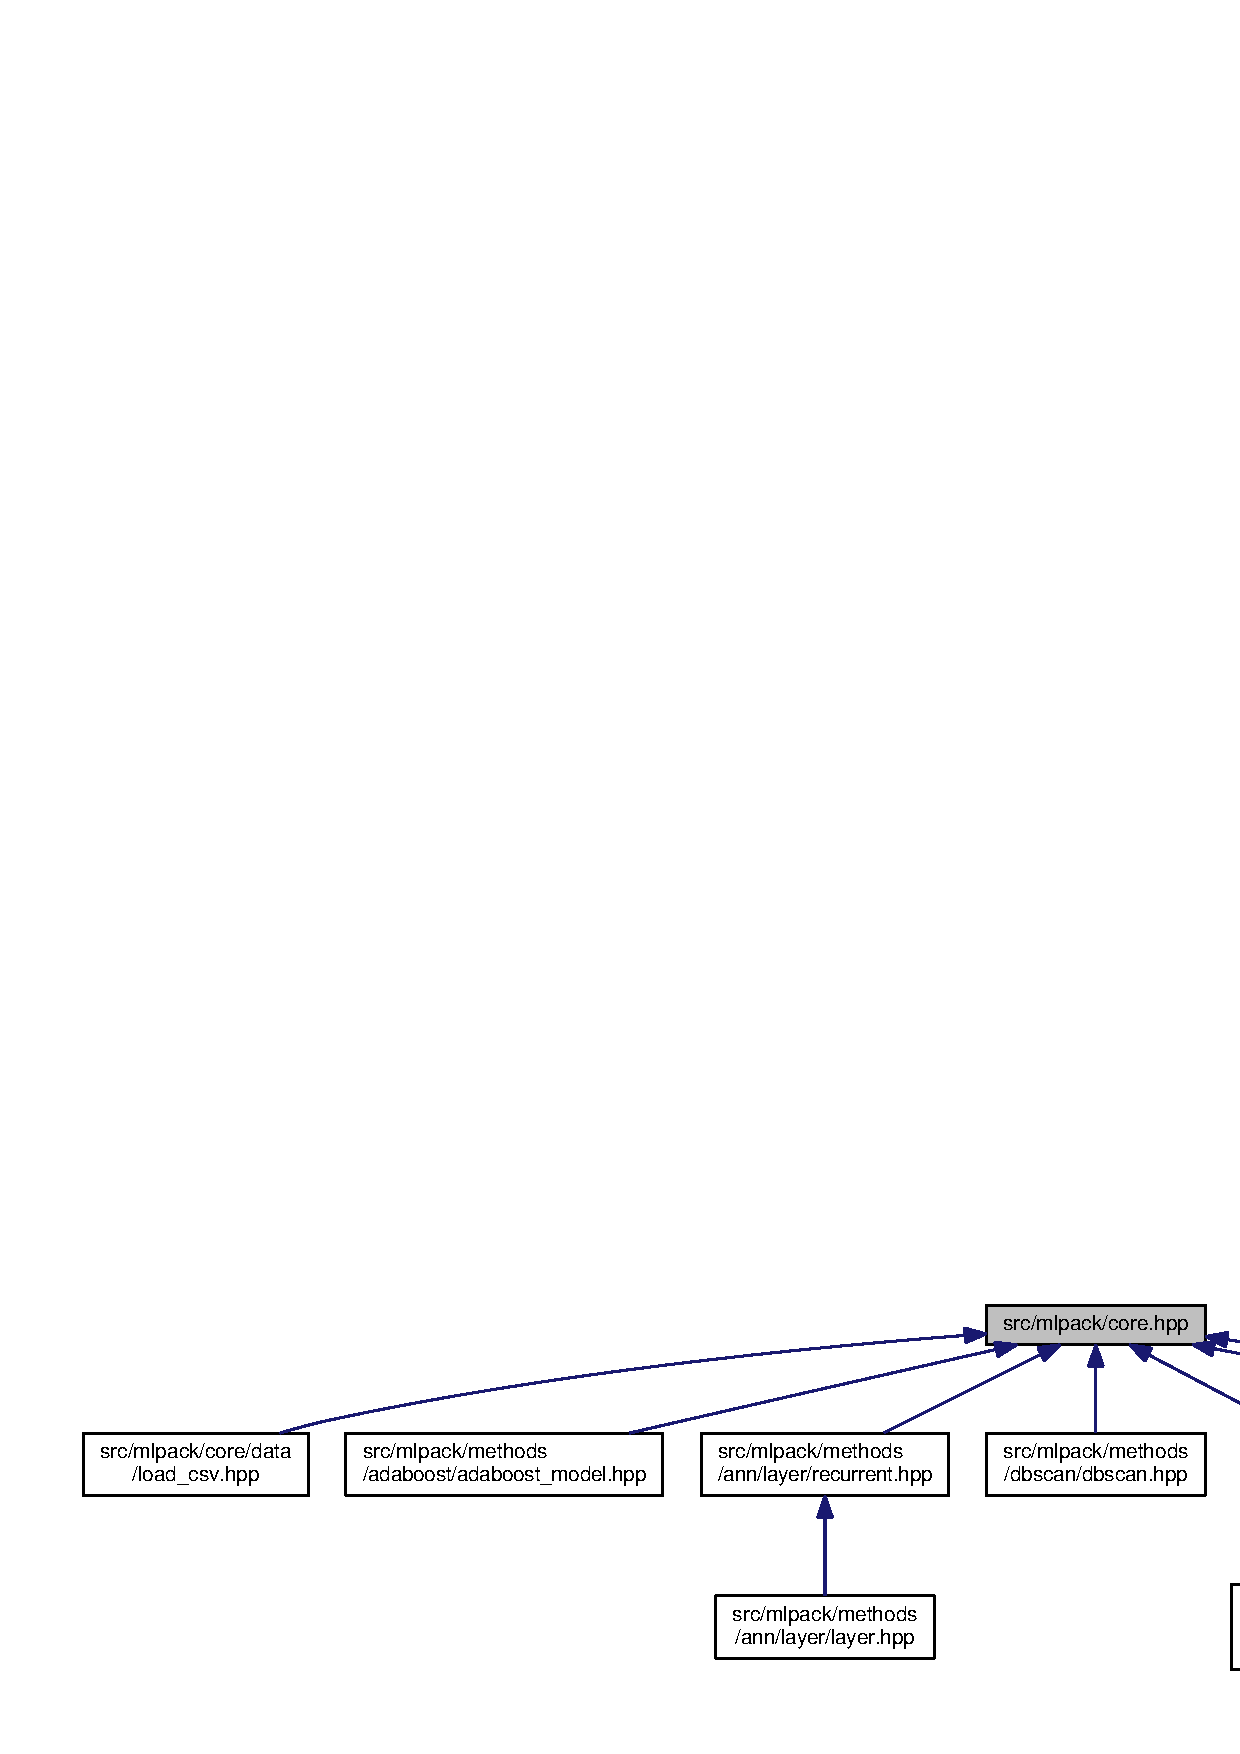
\includegraphics[width=350pt]{core_8hpp__dep__incl}
\end{center}
\end{figure}


\subsection{Detailed Description}
Include all of the base components required to write M\+L\+P\+A\+CK methods, and the main M\+L\+P\+A\+CK Doxygen documentation. 

mlpack is free software; you may redistribute it and/or modify it under the terms of the 3-\/clause B\+SD license. You should have received a copy of the 3-\/clause B\+SD license along with mlpack. If not, see {\tt http\+://www.\+opensource.\+org/licenses/\+B\+S\+D-\/3-\/\+Clause} for more information. 